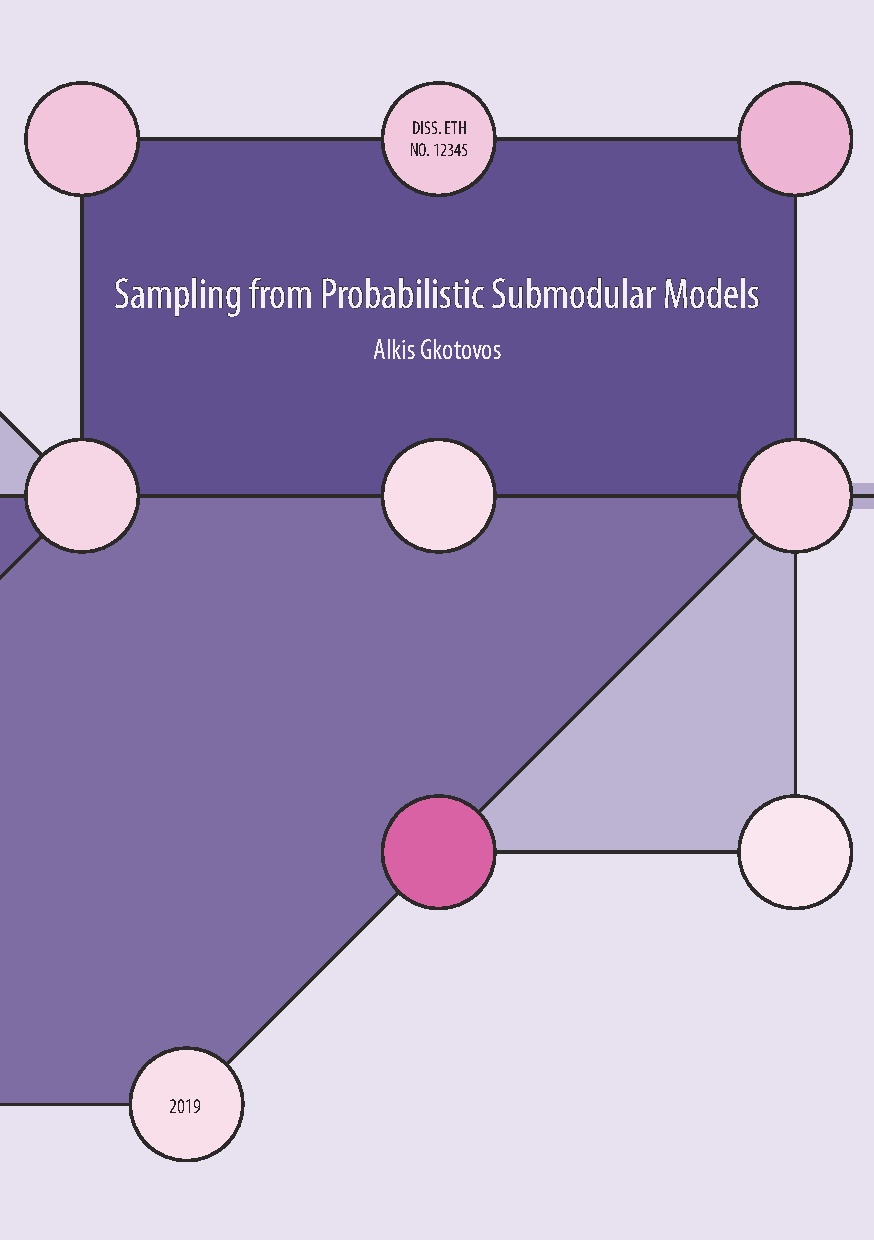
\includepdf[pages={1}]{title/outer.pdf}
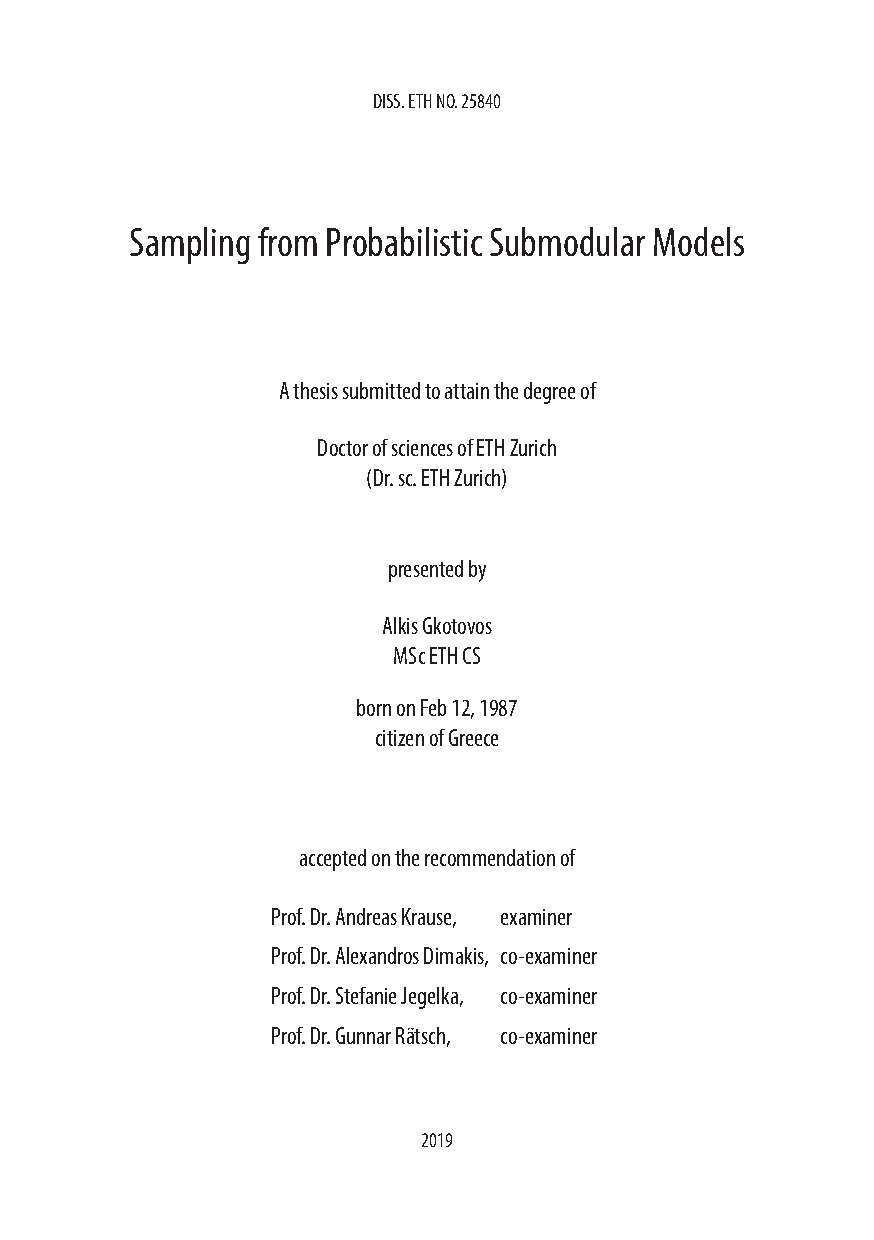
\includepdf[pages={1}]{title/inner.pdf}

\cleardoublepage
\section*{\centering Abstract}
\vspace{1em}
Practical problems of discrete nature are very common in machine learning; application domains include computer vision (e.g., image segmentation), sequential decision making (e.g., active learning), social network analysis (e.g., influence maximization), and natural language processing (e.g., document summarization).
Submodular set functions have found wide applicability in such problems for their ability to capture notions of coverage, diversity, or exclusivity; analogously, supermodular set functions have been used to capture notions of regularity, smoothness, or co-occurrence.

While the topic of submodular optimization has received much attention, these functions can also be used to define expressive discrete probabilistic models, called probabilistic submodular models.
Going beyond optimization, these models allow us to quantify predictive uncertainty, and suggest a maximum likelihood approach for learning such functions from noisy data.
Prominent examples of probabilistic submodular models include Ising and Potts models, as well as determinantal point processes, but the general class is much richer and little studied.

It is well known, though, that performing probabilistic inference in such models is computationally intractable in general.
In this thesis, we investigate the use of Markov chain Monte Carlo sampling as a means of performing approximate inference in probabilistic submodular models.

We start with analyzing the Gibbs sampler, and establish theoretical conditions that guarantee efficient convergence of this sampler in probabilistic submodular models.
We next propose a novel sampling procedure that makes use of discrete semigradients to perform efficient global moves, so as to avoid so-called state-space bottlenecks, and thus lead to improved convergence behavior.
Finally, we employ the aforementioned sampling methods to approximate the likelihood gradients, and learn such models from data.
More specifically, we apply our learning procedure to the problem of modeling interactions between genetic mutations in cancer patients, and demonstrate considerable improvement over the state of the art in many of our experimental results on both synthetic and real cancer data.

\cleardoublepage
\section*{Zusammenfassung}

\cleardoublepage
\section*{Acknowledgements}
\todo{}